% \begin{frame}
%     \frametitle{Visualizzare ed Elaborare documenti XML}
%     \addtocounter{nframe}{1}
    
%     %\begin{center}
%     %    
\includegraphics[width=.2\textwidth]{../imgs/tei-r.pdf}
%     %\end{center}
%     %\textit{In parte già disponibili nei moduli TEI di base}

%      \begin{block}{Perché visualizzare il testo}
%     %     \emph{Per la critica testuale indispensabili i moduli}
%          \begin{itemize}
%             \item  Controllare la codifica e correggere i refusi
%              \item Assicurarsi che tutto sia stato trascritto correttamente
%              \item Mostrare il testo a persone che non conoscono XML-TEI
%              \item Disporre di una versione del lavoro fuibile
%         \end{itemize}
%      \end{block}
    
% \end{frame}

% \begin{frame}
%     \frametitle{Visualizzare ed Elaborare documenti XML}
%     \addtocounter{nframe}{1}
    
%     \begin{center}
%         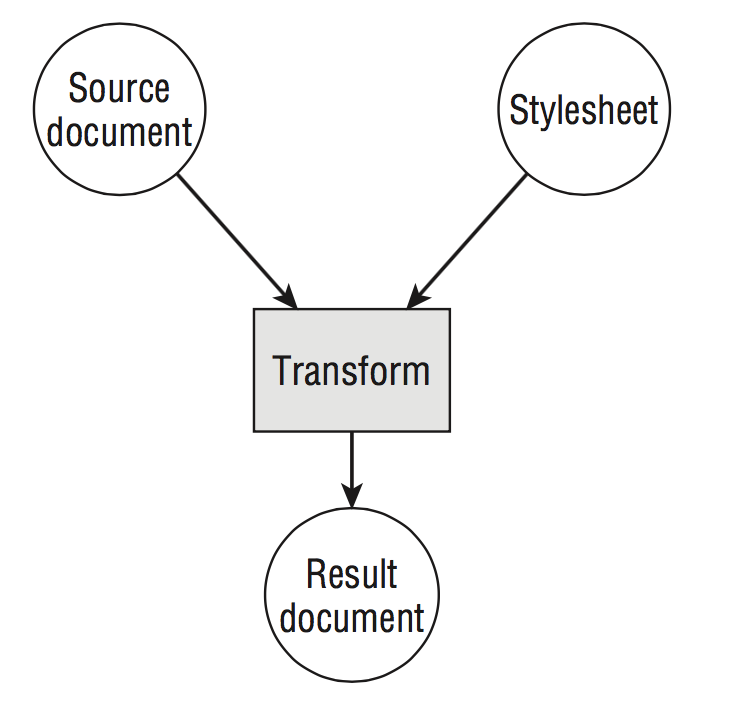
\includegraphics[width=.9\textwidth]{imgs/SchemaXSLTprocessing.png}
%     \end{center}
%     %\textit{In parte già disponibili nei moduli TEI di base}

% \end{frame}

% Controllo e gestione degli spazi bianchi p 54 slide di Chiara

\begin{frame}
    \frametitle{Visualizzare ed Elaborare documenti XML}
    \addtocounter{nframe}{1}
    
    %\begin{center}
    %    
\includegraphics[width=.2\textwidth]{../imgs/tei-r.pdf}
    %\end{center}
    %\textit{In parte già disponibili nei moduli TEI di base}

     \begin{block}{XSLT: come procedere per un buon risultato}
    %     \emph{Per la critica testuale indispensabili i moduli}
         \begin{itemize}
            \item Tracciare una mappa della conversione da XML a (X)HTML
             \item Lasciare il \texttt{<teiHeader>} per ultimo
             \item Definire lo scheletro HTML sul primo \textbf{template rule} e controllare che funzioni
        \end{itemize}
     \end{block}
    
\end{frame}

\begin{frame}
    \frametitle{Visualizzare ed Elaborare documenti XML}
    \addtocounter{nframe}{1}
    
    %\begin{center}
    %    
\includegraphics[width=.2\textwidth]{../imgs/tei-r.pdf}
    %\end{center}
    %\textit{In parte già disponibili nei moduli TEI di base}

     \begin{block}{XSLT: come procedere per un buon risultato}
    %     \emph{Per la critica testuale indispensabili i moduli}
         \begin{itemize}
             \item Divisione strutturale: uso di intestazioni (\texttt{<h1>, <h2> ecc.}) e
             paragrafi, a capo (\texttt{<p>, <br/>}) in HTML
             \item Formattazione degli elementi: usate gli elementi già presenti in
             HTML (\texttt{<b>, <i>, ecc.}) oppure definite degli \texttt{<span>}.
             \item Scrivere una regola alla volta, testarla e solo se funziona passare alla
             successiva
        \end{itemize}
     \end{block}
    
\end{frame}


\begin{frame}
    \frametitle{Visualizzare ed Elaborare documenti XML}
    \addtocounter{nframe}{1}
    
    %\begin{center}
    %    
\includegraphics[width=.2\textwidth]{../imgs/tei-r.pdf}
    %\end{center}
    %\textit{In parte già disponibili nei moduli TEI di base}

     \begin{block}{XSLT: come procedere per XML-TEI}
        Tutti i nomi di elementi TEI devono essere preceduti dal prefisso \textbf{tei:}!
     \end{block}

     \begin{block}{XSLT: come procedere per XML-TEI}
        \texttt{<xsl:stylesheet version="1.0"}
        \\\texttt{ xmlns:xsl="http://www.w3.org/1999/XSL/Transform"}
        \\\texttt{ xmlns:tei="http://www.tei-c.org/ns/1.0"}
        \\\texttt{ xmlns="http://www.w3.org/1999/xhtml" >}
     \end{block}
    
\end{frame}

   

\begin{frame}
    \frametitle{Visualizzare ed Elaborare documenti XML}
    \addtocounter{nframe}{1}
    
    %\begin{center}
    %    
\includegraphics[width=.2\textwidth]{../imgs/tei-r.pdf}
    %\end{center}
    %\textit{In parte già disponibili nei moduli TEI di base}

     \begin{block}{Fogli di stile TEI}
        Gli sviluppatori della TEI mettono a disposizione dei fogli di stile per documenti TEI P4 e posteriori
        \\\texttt{http://www.tei-c.org/Tools/Stylesheets/}
     \end{block}

     \begin{block}{XSLT per XML-TEI}
        \texttt{http://sourceforge.net/projects/tei/}
        \\\texttt{http://tei.oucs.ox.ac.uk/teideb/binary}
        \\\texttt{http://www.tei-c.org/oxgarage/}
        \\\texttt{http://wiki.tei-c.org/index.php/Stylesheets}
        \\\texttt{git hub TEI/TEIC}
     \end{block}
    
\end{frame}


\begin{frame}
    \frametitle{Visualizzare ed Elaborare documenti XML}
    \addtocounter{nframe}{1}
    
    %\begin{center}
    %    
\includegraphics[width=.2\textwidth]{../imgs/tei-r.pdf}
    %\end{center}
    %\textit{In parte già disponibili nei moduli TEI di base}

     \begin{block}{Riferimenti}
            \begin{itemize}
                \item Michael Kay, XSLT 2.0 and XPath 2.0 Programmer's Reference
                \item James Clark, XSL Transformations (XSLT) Version 1.0, W3C Recommendation 16 November 1999, http://www.w3.org/TR/xslt
                \item E.R. Harold, XSL Transformations (XSLT), capitolo 14 del libro XML
                Bible, disponibile in rete:
                \item[] \url{http://metalab.unc.edu/xml/books/bible/updates/14.html} 
            \end{itemize}
     \end{block}
    
\end{frame}


